\section{Theory background}
This section provides the required theoretical background on GANs in general and Wasserstein GAN in particular. 
\subsection{Generative adversarial networks (GANs)}
The goal of generative adversarial networks is to produce realistic data samples by learning from a given data set $D$. This can be accomplished by learning the underlying probability distribution of the data set $P_r$, the "real" probability distribution.

There are two approaches for learning $P_r$:
\begin{enumerate}
	\item To learn $P_r$ directly by defining a parametrized $P_\theta$ and finding parameters $\theta$ using the \textit{maximum likelihood estimation} (MLE)
	\item To use an input noise variable $z$ with a known probability density function $p_z(z)$ and define a parametrized mapping function $g_\theta: Z \rightarrow D$. Then, the density function of generated samples in denoted by $p_g(g_\theta(z))$. 
\end{enumerate}

While the first approach seems more straightforward, there are some flows in it. Maximizing the mean logarithm of the objective function $MLE(\theta)$ is equivalent to minimizing the \textit{Kullback-Leibler divergence}\footnote{Kullback-Leiber divergence is a measure of how one probability distribution divergence from a second one and is defined by $KL(P \lVert Q) = \int_{x} p(x) \log \frac{p(x)}{q(x)} dx$} between the two distributions $KL(P_r \lVert P_\theta)$:

\begin{align*}
	\lim_{m \to \infty} \max_{\theta} \frac{1}{m} \log MLE(\theta)
	&= \max_\theta \int_x p_r(x) \log p_\theta(x) dx \\
	&= \min_\theta - \int_x p_r(x) \log p_\theta(x) dx \\
	&= \min_\theta \int_x p_r(x) \log p_r(x) dx - \int_x p_r(x) \log p_\theta(x) dx \\
	&= \min_\theta KL(P_r \lVert P_\theta)
\end{align*}

If there is at least one data point $x \in P_r$ which has $p_\theta(x) = 0$, then the KL-divergence will immediately be infinitely large. This is a common scenario in practice, because $P_\theta$ tries to find a low dimensional manifold in the space of the observed data, and there are points lying outside of this manifold. In practice, a workaround to this problem is to add noise term $\epsilon$ to the model, to make sure that $P_\theta$ is defined everywhere. Then, the estimated probability distribution will be defined by 
\begin{equation*}
p_{estimated}(x) = \frac{p_\theta(x) + \lambda \cdot \epsilon(x)}{\int_x p_\theta(x) + \lambda \cdot \epsilon(x) dx}, 
\end{equation*}
where $\lambda$ is the amount of noise we want to add to the model. This, however, is not an ideal solution because it degrades the sample quality. \\
  
\indent Generative adversarial networks implement the latter approach with a mapping function $g_\theta$ being encoded using a neural network, called \textit{generator} $G$. Instead of the MLE generative adversarial networks use \textit{adversarial training} to find parameters for the generator. To measure the quality of the generator $G$ another network is used, the \textit{discriminator}, which takes an input sample and outputs the probability that the sample comes from the real data set. The architecture of a GAN is shown in Figure~\ref{fig:gan}.\\

\begin{figure}[h]
	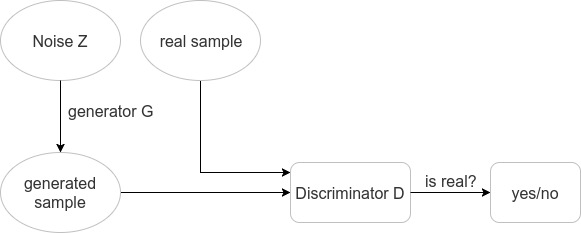
\includegraphics[width=\textwidth]{figures/gan}
	\caption{A visualization of how different parts of a GAN are connected with each other. A generator network $G$ produces samples from a noise variable $Z$. A discriminator network $D$ takes both real and generated samples and tries to distinguish between them.}
	\label{fig:gan}
\end{figure}

\indent In order to train a GAN model one has to define two loss functions. One that quantifies how well a discriminator $D$ can distinguish between a real probability distribution $p_r(x)$ and its approximation computed by a generator $G$, $p_g(G(z))$. Second loss function evaluates how well the generator can approximate the real distribution. For a standard GAN these loss functions are defined as: 
\begin{equation} \label{eq:gan_loss}
\argmin_G \argmax_D L(G,D) = \E_{x \sim p_r(x)} [\log(D(x)] + \E_{z \sim p_z(z)}[\log(1-D(G(z))]
\end{equation}
Let us analyze equation~\ref{eq:gan_loss} from the viewpoint of a discriminator. The maximum value of $L(G,D)$ is achieved when both $\E_{x \sim p_r(x)} [\log D(x)]$ and $\E_{z \sim p_z(z)}[\log(1-D(G(z)))]$ are equal to zero. For this to hold, the values inside of the  logarithms should be equal to one. This means that the discriminator should output one for real samples and zero for generated ones. When optimizing with respect to the generator the first term of equation~\ref{eq:gan_loss} is constant. And the term $\E_{z \sim p_z(z)}[\log(1-D(G(z))]$ is equal to zero when the discriminator thinks that the samples generated by the generator are real. There is no closed form solution for~\ref{eq:gan_loss} and the most common method of optimization is by applying a gradient descent to the generator and to discriminator alternately.\\  

\indent A natural question that arises after looking at the adversarial training procedure is how it relates to measuring distance between the real distribution $P_r$ and the generated one $P_G$. 

First observation is that with a generator $G$ fixed, optimal discriminator $D$ is equal to
\begin{equation}
	D^*(x) = \frac{p_r(x)}{p_r(x) + p_g(x)}
\end{equation}
\begin{proof}
	\begin{align*}
		L(G, D) &= \int_x p_r(x)\log(D(x))dx + \int_z p_z(z)\log(1 - D(G(z))) dz \\
		&= \int_x p_r(x)\log(D(x))dx + \int_x p_g(x)\log(1 - D(x)) dx
	\end{align*}
The minimal value of a function $a\log(y) + b\log(1-y)$ is achieved at the point $y = \frac{a}{a+b}$ for all $(a,b) \in \mathbb{R}^2 \setminus (0,0)$. This can be shown by finding a null point of the corresponding derivative $\frac{a}{y} - \frac{b}{1-y}$.
\end{proof}

Now with an optimal discriminator $D^*$ we can rewrite $L(G,D)$ as following
\begin{align*}
	L(G, D) &= \E_{x \sim p_r(x)} [\log(D^*(x)] + \E_{z \sim p_z(z)}[\log(1-D^*(G(z))] \\
	&= \E_{x \sim p_r(x)} [\log(D^*(x)] + \E_{x \sim p_g}[\log(1-D^*(x)] \\
	&= \E_{x \sim p_r(x)} \bigg[\log \frac{p_r(x)}{p_r(x) + p_g(x)}\bigg] + \E_{x \sim p_g}\bigg[\log \frac{p_g(x)}{p_r(x) + p_g(x)}\bigg] \\
	&= -\log 4 + \E_{x \sim p_r(x)} \bigg[\log \frac{p_r(x)}{\frac{p_r(x) + p_g(x)}{2}}\bigg] + \E_{x \sim p_g}\bigg[\log \frac{p_g(x)}{\frac{p_r(x) + p_g(x)}{2}}\bigg] \\
	&= -\log 4 + KL\bigg(P_r \lVert \frac{P_r + P_g}{2}\bigg) +  KL\bigg(P_g \lVert \frac{P_r + P_g}{2}\bigg) \\
	&= -\log 4 + 2 \cdot JSD(P_r \lVert P_g),
\end{align*}
where $JSD(P_r \lVert P_g)$ is the \textit{Jensen-Shannon divergence}  \footnote{Jensen-Shannon divergence is a distance measure between two probability distributions and is defined by $JS(P\lVert Q) = \frac{1}{2} KL(P \lVert \frac{P+Q}{2}) +\frac{1}{2} KL(Q \lVert \frac{P+Q}{2})$, where KL denotes the Kullback-Leibler divergence.} between two distributions. Since the JS divergence is defined everywhere, this approach does not suffer from the problems described for the MLE.

We have shown that assuming that a discriminator is always trained to optimality, objective function defined in equation~\ref{eq:gan_loss} can be interpreted as a Jensen-Shannon divergence between the real distribution $P_r$ and the one approximated by a generator $P_g$.  

The training process of a GAN consists of the following steps:
\begin{enumerate}
	\item With a fixed generator train a discriminator to optimality.
	\item With an optimal discriminator, train the generator. 
	\item Repeat previous steps. Knowing when to stop the training process is not trivial and will be discussed in the following sections.
\end{enumerate}
Since we can not compute $\E_{x \sim p_r(x)} [\log(D(x)]$ we approximate in by 
\begin{equation}
	\frac{1}{m} \sum_{i=1}^{m} D(x_i),
\end{equation}
where $x_i$ is a random subset of training samples, $m$ is usually small compared to the number of training samples available. This technique is called \textit{stochastic gradient descent}. The same is done to compute $\E_{z \sim p_z(z)}[\log(1-D(G(z))]$.
 
\subsection{Wasserstein GANs (WGANs)}
Wasserstein GANs were introduced in January 2017~\citep{wgan}. The authors argue that the Jensen-Shannon divergence, used in original GANs to calculate the distance between generated and original probability distributions, has some problems and proposed a new objective function based on the \textit{Earth-Mover} (EM)  distance. This distance should improve stability of the training process and provide a distance measure that corresponds to the perceived sample quality. 
	The Earth-Mover distance between two distributions is defined by
\begin{equation}
	W(P_g, P_r) =  \inf_{\gamma \in \prod (P_r, P_g)}  \E_{(x,y) \sim \gamma} [ \lVert x - y \lVert_2 ],
\end{equation}
where $\prod (P_r, P_g)$ is a set of all joint distributions $\gamma(x,y)$ whose marginal distributions are $P_r$ and $P_g$ respectively. To understand the idea behind the EM distance we can imagine that probability distributions assign a mass to each point $x$ and we want to turn distribution $P_r$ into $P_g$ by moving this mass around. Furthermore, moving a mass $m$ by a distance $d$ would cost us $m \cdot d$ effort. In this imaginary scenario the EM distance will give us the minimal effort we would have to spend. Why is this true? 
\begin{itemize}
	\item We can think of each $\gamma(x, y)$ as the amount of mass transported between points $x$ and $y$, then in our scenario $\gamma$ will represent a "transport plan" for transitioning from $P_r$ to $P_g$.
	\item For $\gamma$ to be a valid strategy it has to satisfy several conditions:
		\subitem Amount of mass leaving point $x$ is calculated by $\int_y \gamma(x, y) dy$ and should be equal to $p_r(x)$, the amount of mass originally located at $x$
		\subitem In the same way, the amount of mass entering $y$ is calculated by $\int_x \gamma(x, y) dx$ and should be equal to $p_g(y)$, the amount of mass located at $y$ at the end.
	\item These conditions mean that marginal distributions of $\gamma(x, y)$ should equal to $P_r$ and $P_g$ respectively. 
	\item The amount of effort required to execute the transporting plan $\gamma$ is 
	\begin{equation}
	\int_x \int_y \gamma(x,y) \lVert x - y \lVert_2 dx dy = \E_{(x,y) ~\sim \gamma} [ \lVert x - y \lVert_2 ]
	\end{equation}
	\item Infinum over this effort gives the EM distance. 
\end{itemize}

One property that is expected from an objective function is that it is continuous and differentiable in its whole domain. And this is exactly where EM distance outperforms the Jensen-Shannon divergence, which is illustrated in the following example, taken from the original paper. 

Consider a uniform random variable $Z \in [0, 1]$. Let $P_r$ be the distribution of a random variable $(0, Z) \in \mathbb{R}^2$. Let $g_\theta: \mathbb{R} \rightarrow \mathbb{R}^2$, $g_\theta(z) = (\theta, z)$ be a mapping function with a single parameter $\theta$. Now we can compute the Jensen-Shannon divergence and the EM distance between $P_r$ and $P_g$. 
To compute the Jensen-Shannon divergence we first need to compute $KL(P_r \lVert M)$ where $M = \frac{1}{2}P_r + \frac{1}{2}P_g$:
\begin{equation}
	KL(P_r \lVert M) = \int_{x,y} p_r(x,y) \log \frac{p_r(x,y)}{m(x,y)} dxdy = \log2,
\end{equation}
because $m(x,y) = \frac{1}{2} p_r(x,y)$ everywhere except for points with $x=0$ or $x=\theta$. The same is true for $KL(P_g \lVert M)$ and therefore:
\begin{align*}
 JSD(P_r \lVert P_g) &= \frac{1}{2}KL(P_r \lVert M) + \frac{1}{2}KL(P_g\lVert M) \\ 
 	&= \begin{cases}
 		\log2, & \text{if } \theta \neq 0 \\
 		0, & \text{if } \theta = 0
 	\end{cases}.
\end{align*}  
On the other hand, if we recall the example explaining the intuition behind the ME distance, we can see that to transport all the mass from $P_r$ to $P_\theta$ we need to transport each mass point by distance $\theta$, therefore
\begin{equation}
	M(P_r, P_g) = \int_{(0,z)} |\theta| \cdot p_r(0,z)dz = |\theta|
\end{equation}

Already from this example we can see that there are cases where the EM distance is continuous whilst JS divergence not. Authors have shown that if a mapping function $g_\theta(x)$ is itself continuous, so that is the EM distance $M(P_r, P_g)$. Moreover, if $g_\theta(x)$ fulfills certain criteria, EM distance will be differentiable almost in the whole domain. At the same time, both statements are false for the JS divergence~\citep{wgan}. The criteria for the function $g_\theta(x)$ to be fulfilled are:
\begin{enumerate}
	\item The function $g_\theta$ is \textit{locally Lipschitz continuous}. \\
	A real-valued function $g_\theta$ is called Lipschitz continuous if there exists a constant $K$, called a \textit{Lipschitz constant}, such that for all $x_1$ and $x_2$:
	\begin{equation}
		\lVert g_\theta(x_1) - g_\theta(x_2) \lVert_2 \leq K\lVert x_1 - x_2 \lVert_2
	\end{equation}  
	Local Lipschitz continuity means that for each point $x$ there exists a neighborhood $U$ where $g_\theta$ is Lipschitz continuous. \\
	In other words, Lipschitz continuity restricts how fast a function can change, because the inclination angle of the line connecting \textbf{each} two points of the function(and thus the value of derivatives) is restricted by a constant $K$. 
	\item The function $g_\theta$ satisfies \textit{regularity assumption 1}. \\
	Let $K(\theta, z)$ denote the local Lipschitz constant at point $(\theta, z)$ of a locally Lipschitz continuous function $g_\theta(z)$. Then, $g_\theta$ satisfies the regularity assumption 1 if the expected value of $K(\theta, z)$ is upper-bounded:
	\begin{equation}
		\E_z[K(\theta, z)] < +\infty
	\end{equation}
\end{enumerate} 
While these assumptions are tedious to prove manually for each mapping function $g_\theta$, authors have shown that all feed-forward neural networks with pointwise or rectified nonlinearities satisfy both these requirements and therefore when using such networks to encode a  generator of a GAN, the EM distance will be continuous and differentiable almost everywhere.  

To utilize the properties of the EM distance we should be able to compute it efficiently. Unfortunately, computing it exactly is not feasible, therefore we have to approximate. 
Firstly, we can use the Kantorovich-Rubinstein duality to rewrite $W(P_r, P_\theta)$ as following
\begin{equation}
	W(P_r, P_\theta) = \sup_{\lVert f \lVert_L \leq 1} \E_{x \sim P_r}[f(x)] - E_{x \sim P_\theta} [f(x)],	
\end{equation}
where ${\lVert f \lVert_L \leq 1}$ denotes the set of all functions that are Lipschitz continuous with Lipschitz constant equal $1$, or also called \textit{1-Lipschitz} functions. If we replace this set with ${\lVert f \lVert_L \leq K}$ we will receive the upper bound for $K \cdot W(P_r, P_\theta)$ instead, which is still intractable to compute but easier to approximate. As already discussed, a discriminator $D$  encoded using a neural network with parameters $w$ is a $K$-Lipschitz function. Therefore
\begin{align*}
\max_w \E_{x \sim P_r}[D(x)] - E_{x \sim P_\theta} [D(x)] &\leq \sup_{\lVert D \lVert_L \leq K} \E_{x \sim P_r}[D(x)] - E_{x \sim P_\theta} [D(x)] \\
 &= K \cdot W(P_r, P_\theta)
\end{align*}
Note, that supremum may not be achieved, if there is a $K$-Lipschitz function that can not be encoded with parameters $\theta$ or if the supremum is achieved for some $k$-Lipschitz function with $k < K$.

One thing that is remained to do is to ensure that $K$ remains constant during the training process. One obvious way to do that is to restrict the space $S$ of possible functions encoded by $D$, then the set of possible Lipschitz constants will be upper-bounded. We enforce discriminators to lie in $S$ by defining an upper and a lower bound for all weights of a discriminant, which will remain unchanged throughout the training process. This process is called \textit{weight clipping}.
 
To train the discriminator we have to compute the gradients of $W(P_r, P_\theta)$ with respect to $w$:
\begin{align*}
	\nabla_w W(P_r, P_\theta) &= \nabla_w(\E_{x \sim P_r}[D_w(x)] - E_{z \sim Z} [D_w(G_\theta(z))]) \\
&= \E_{x \sim P_r}[\nabla_w(D_w(x))] - \E_{z \sim Z} [\nabla_w(D_w(G_\theta(z)))]
\end{align*} 
In the same way, updates for Generator $G$ are obtained by computing the gradients with respect to $\theta$ 
\begin{align*}
\nabla_\theta W(P_r, P_\theta) &= \nabla_\theta(\E_{x \sim P_r}[D_w(x)] - E_{z \sim Z} [D_w(G_\theta(z))]) \\
&= - \E_{z \sim Z} [\nabla_\theta D_w(G_\theta(z))]
\end{align*}

The training process therefore consists of the following steps:
\begin{enumerate}
	\item For a fixed generator train the discriminator to the convergence in order to obtain an approximation of $W(P_r, P_\theta)$:
	\begin{enumerate}
		\item Update discriminator's weights using computed gradient.
		\item Enforce the discriminator to remain $K$-Lipschitz by clipping its to values $[-c, c]$, where $c$ remains constant during the training process.
	\end{enumerate}	
	\item With an optimal discriminator update the generator by computing the gradient $- \E_{z \sim Z} [\nabla_\theta D(G(z))]$	
\end{enumerate}

\begin{figure}[h!]
  \begin{subfigure}[b]{0.5\textwidth}
    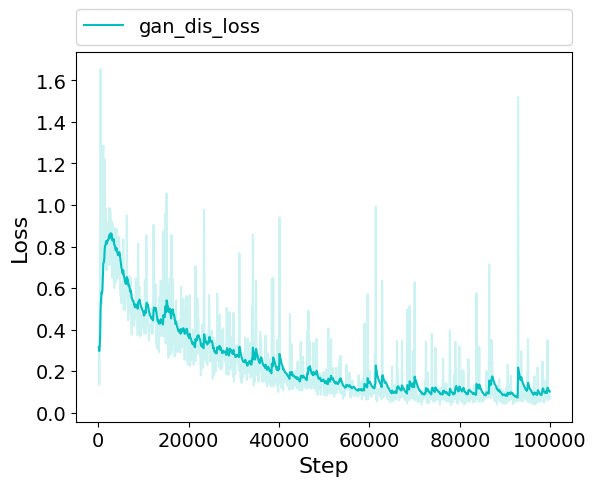
\includegraphics[width=\textwidth]{figures/ex/gan_dis_loss}
    \caption{GAN discriminator loss}
    \label{fig:gan_dis_loss}
  \end{subfigure}
  \hfill
  \begin{subfigure}[b]{0.5\textwidth}
    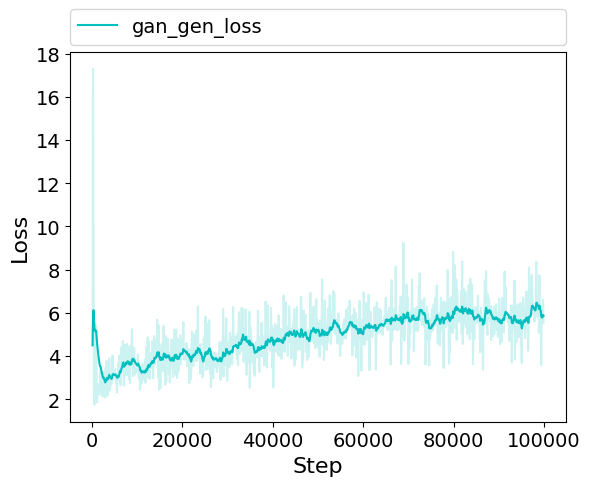
\includegraphics[width=\textwidth]{figures/ex/gan_gen_loss}
    \caption{GAN generator loss}
    \label{fig:gan_gen_loss}
  \end{subfigure}
  \begin{subfigure}[b]{0.5\textwidth}
    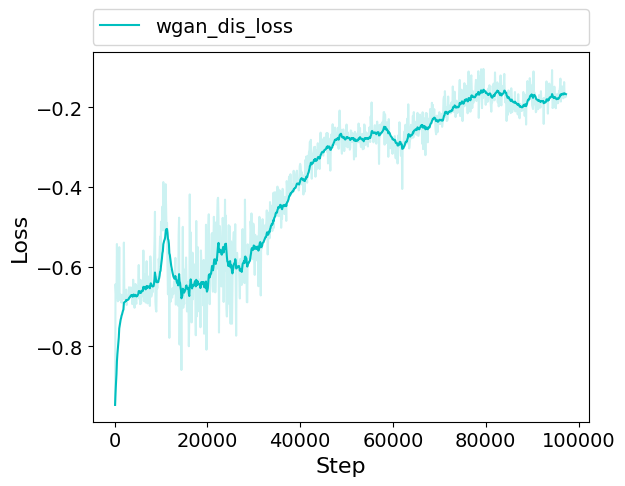
\includegraphics[width=\textwidth]{figures/ex/wgan_dis_loss}
    \caption{Wasserstein GAN discriminator loss}
    \label{fig:wgan_dis_loss}
  \end{subfigure}
  \hfill
  \begin{subfigure}[b]{0.5\textwidth}
    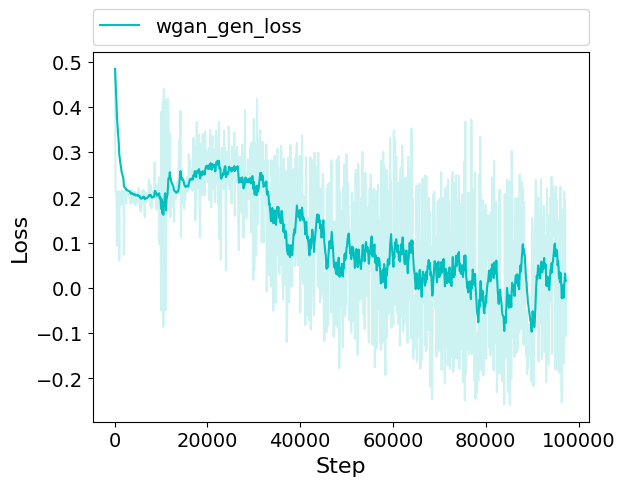
\includegraphics[width=\textwidth]{figures/ex/wgan_gen_loss}
    \caption{Wasserstein GAN generator loss}
    \label{fig:wgan_gen_loss}
  \end{subfigure}
  
  \caption{Figures illustrating that WGAN has a correlation between the number of training steps and the values of its objective functions. On the other hand the loss of the GAN generator increases although the quality of the produced images increases too.}
  \label{fig:losses}
\end{figure}
\begin{figure}[h]
  \begin{subfigure}[b]{\textwidth}
    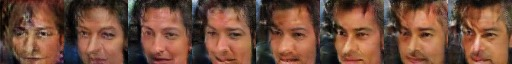
\includegraphics[width=\textwidth]{figures/gan_progress}
    \caption{Evolution of GAN generated samples quality}
    \label{fig:gan_evolution}
  \end{subfigure}
  \begin{subfigure}[b]{\textwidth}
    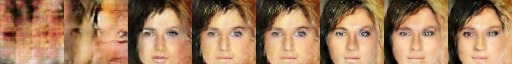
\includegraphics[width=\textwidth]{figures/wgan_progress}
    \caption{Evolution of Wasserstein GAN generated samples quality}
    \label{fig:gan_evolution}
  \end{subfigure}
  \caption{Samples generated after different number of training steps. Each sample is generated from the same noise variable.}
  \label{fig:samples_evolution}
\end{figure}

Apart from the fact that the Wasserstein GAN allows more stable training, its loss function corresponds to the image quality. This is illustrated in Figures~\ref{fig:losses} and~\ref{fig:samples_evolution}.



\subsection{Deep Convolutional GANs (DCGANs)}
So far we discussed GANs without paying attention to the architecture of underlying generator and discriminator. On the one hand, this is a powerful feature of the framework, because it allows a higher level of abstraction. It is possible to encode a generator and a discriminator using a deep convolutional neural network, an auto-encoder or every other network type. However, this choice inevitably affects the performance of the resulting GAN and therefore has to be thoroughly evaluated. In my thesis I have used deep convolutional GANs (DCGANs) because they are well suited for image generation tasks~\cite{dcgan}. In DCGANs both a generator and a discriminator are encoded convolutional neural networks (CNNs) and this section provides an overview of this network type. 

First introduced in their current form in 1996 by Yann LeCunn~\cite{lecun}, CNNs became really popular in 2012, when a CNN called AlexNet won an image recognition competition significantly improving all previous results~\cite{alexnet}. 


\begin{figure}[h]
  \begin{subfigure}[b]{0.24\textwidth}
    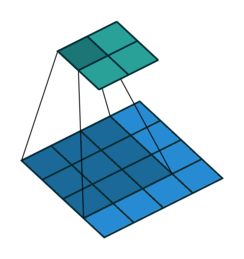
\includegraphics[width=\textwidth]{figures/no_padding_no_strides_00}
  \end{subfigure}
  \begin{subfigure}[b]{0.24\textwidth}
    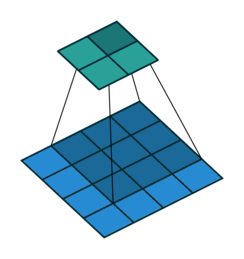
\includegraphics[width=\textwidth]{figures/no_padding_no_strides_01}
  \end{subfigure}
  \begin{subfigure}[b]{0.24\textwidth}
    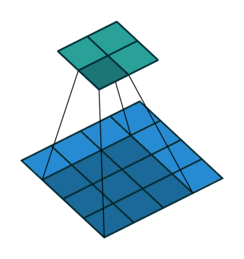
\includegraphics[width=\textwidth]{figures/no_padding_no_strides_02}
  \end{subfigure}
  \begin{subfigure}[b]{0.24\textwidth}
    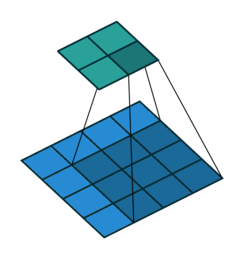
\includegraphics[width=\textwidth]{figures/no_padding_no_strides_03}
  \end{subfigure}  
  \caption{An example of a convolution filter. The lower matrix is an input layer, the upper one represents the output layer. The patches being convoluted are highlighted with a darker color.}
  \label{fig:conv_no_padding_no_strides}
\end{figure}

The core idea of CNNs is to learn hierarchies of location independent features present in an image. Features in the first layer of a CNN are just geometric primitives like edges, but last layers represent complex context dependent features like eyes or noses. Layers of a CNN are built of multiple \textit{convolution filters} that are applied to each patch of the input, as shown\footnote{All visualizations of convolution filters where generated using the code provided by the author of the paper~\cite{conv_tutorial}. The code is available on GitHub: \url{https://github.com/vdumoulin/conv_arithmetic}.} in Figure~\ref{fig:conv_no_padding_no_strides}. A convolution filter $F \in \mathbb{R}^{K \times K}$ is a matrix of weights. When applying $F$ to a patch $P$ of the input we simply compute the sum of the element-wise product between $F$ and $P$:

\begin{equation}
	F * P  = \sum_{i=1}^K \sum_{j=1}^K f_{ij} \cdot p_{ij}.
\end{equation}

\begin{figure}[h!]
  \begin{subfigure}[b]{0.32\textwidth}
    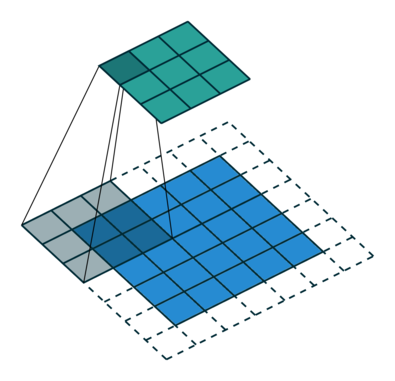
\includegraphics[width=\textwidth]{figures/padding_strides_00}
  \end{subfigure}
  \begin{subfigure}[b]{0.32\textwidth}
    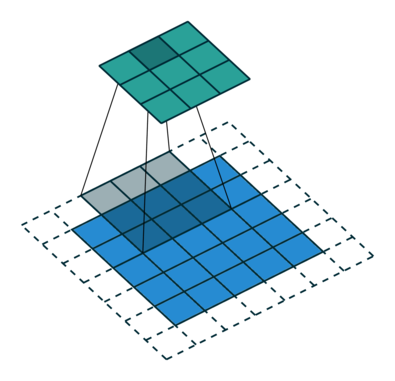
\includegraphics[width=\textwidth]{figures/padding_strides_01}
  \end{subfigure}
  \begin{subfigure}[b]{0.32\textwidth}
    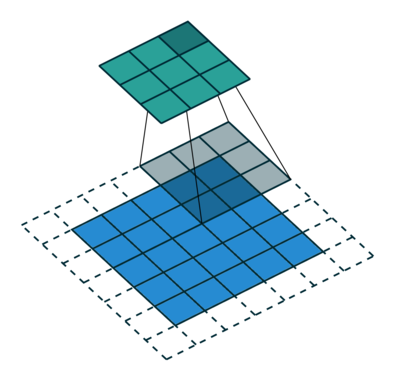
\includegraphics[width=\textwidth]{figures/padding_strides_02}
  \end{subfigure}
%  \begin{subfigure}[b]{0.32\textwidth}
%    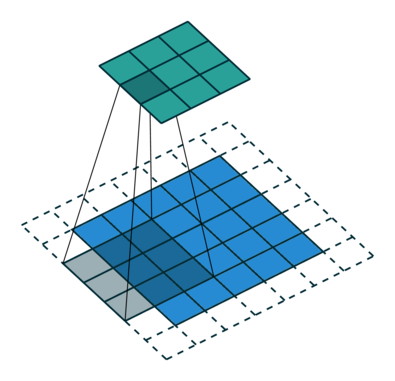
\includegraphics[width=\textwidth]{figures/padding_strides_03}
%  \end{subfigure}  
%  \begin{subfigure}[b]{0.32\textwidth}
%    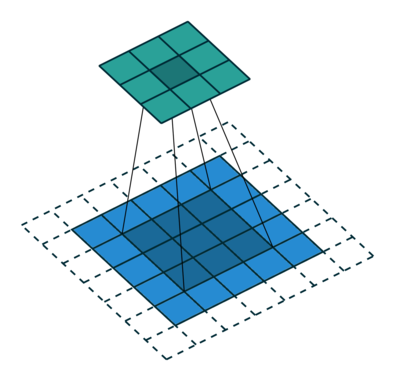
\includegraphics[width=\textwidth]{figures/padding_strides_04}
%  \end{subfigure}
%  \begin{subfigure}[b]{0.32\textwidth}
%    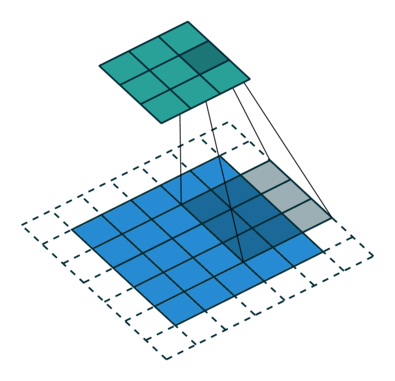
\includegraphics[width=\textwidth]{figures/padding_strides_05}
%  \end{subfigure}
%  \begin{subfigure}[b]{0.32\textwidth}
%    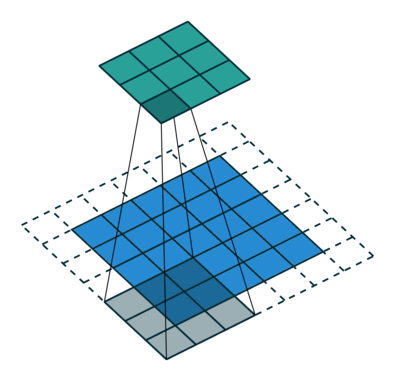
\includegraphics[width=\textwidth]{figures/padding_strides_06}
%  \end{subfigure}
%  \begin{subfigure}[b]{0.32\textwidth}
%    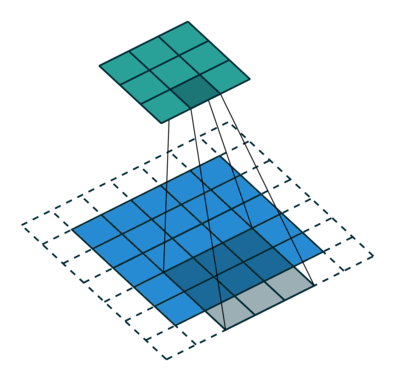
\includegraphics[width=\textwidth]{figures/padding_strides_07}
%  \end{subfigure}  
%  \begin{subfigure}[b]{0.32\textwidth}
%    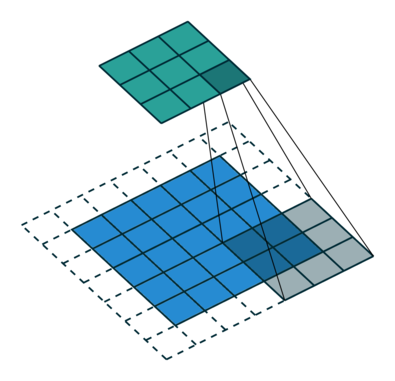
\includegraphics[width=\textwidth]{figures/padding_strides_08}
%  \end{subfigure}  
  \caption{An example of a convolution filter with padding $p=(1,1)$ and strides $s = (2,2)$. The transparent cells of the lower matrix represent padded zero elements.}
  \label{fig:conv_padding_strides}
\end{figure}

Since the same filter $F$ is applied to each patch of the input, it learns a location independent feature present there. Sometimes the input matrix is \textit{padded} with $p$ zeros to increase the number of patches. The distance between the centers of two adjacent patches is called \textit{stride} $s$, as illustrated in Figure~\ref{fig:conv_padding_strides}. Strides and padding allow to manipulate the size of the output:

\begin{equation}
	o = \Bigl\lfloor \frac{i + 2p - k}{s} \Bigr\rfloor + 1,
\end{equation}
where $i$ is the size of the input, $o$ size of the output, $k$ size of the convolution filter, $p$ and $s$ sizes of padding and strides respectively. After a convolution filter some non linear function is applied to the output. In my experiments I have used the leaky rectified linear units(leaky ReLUs): 

\begin{equation}
	f(x) = \begin{cases}
			x & \text{if }x > 0\\
			a \cdot x &\text{otherwise}
			\end{cases}	
\end{equation}

In the DCGAN generator another convolution type is used. It is called \textit{transposed convolution}. The convolution operation can be rewritten as a product of the input and a sparse matrix $C$~\cite{conv_tutorial}. Then, we can transpose $C$ to swap the input and the output. The resulting product of the input and $C^T$ can be again replaced by sliding the convolutional matrix $F$ over the input. An example of a transposed convolution is shown in Figure~\ref{fig:conv_padding_strides_transposed}. Transposed convolutions allow to increase the input dimensions while keeping the same connectivity pattern as in the convolution filter. 

\begin{figure}
	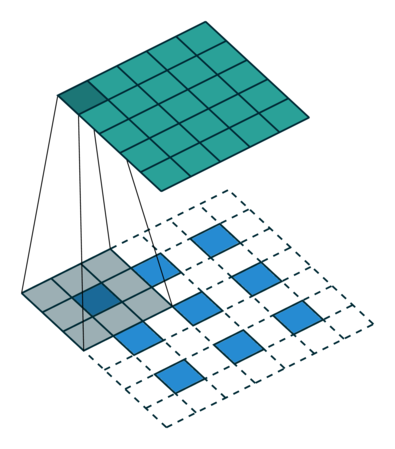
\includegraphics[width=0.18\textwidth]{figures/padding_strides_transposed_00}
	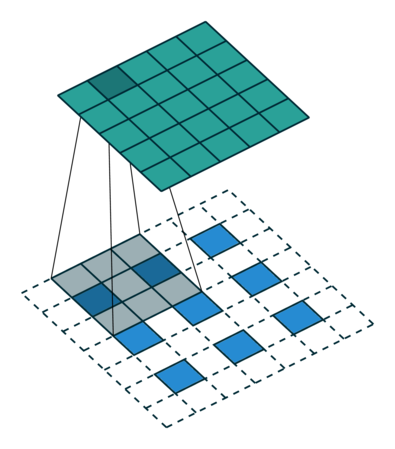
\includegraphics[width=0.18\textwidth]{figures/padding_strides_transposed_01}
	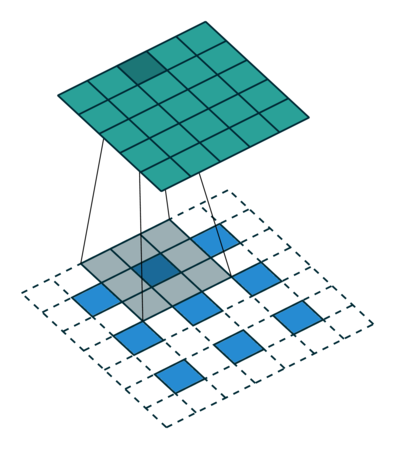
\includegraphics[width=0.18\textwidth]{figures/padding_strides_transposed_02}
	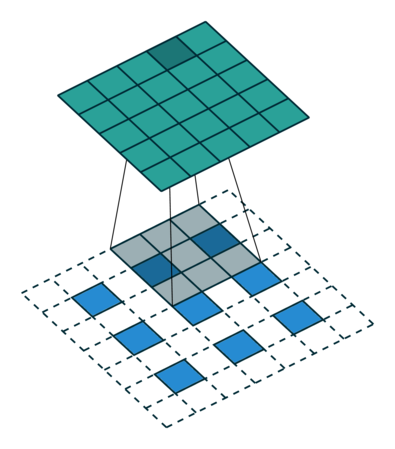
\includegraphics[width=0.18\textwidth]{figures/padding_strides_transposed_03}
	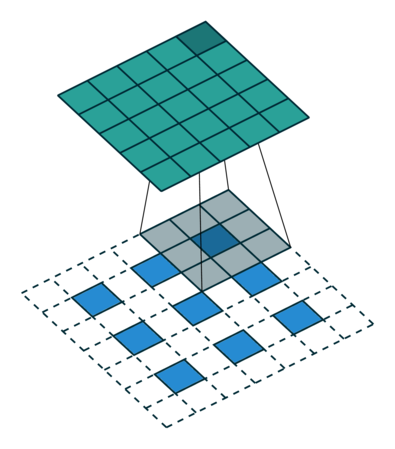
\includegraphics[width=0.18\textwidth]{figures/padding_strides_transposed_04}
	\caption{ The transpose of convolving a kernel $k=(3,3)$ over an input $i=(5,5)$ padded with $p=(1,1)$ border of zeros using strides $s=(2,2)$. It is equivalent to convolving a kernel $\tilde{k} = (3,3)$ over an input $\tilde{i} = (3,3)$ (with 1 zero inserted between inputs) padded with $p=(1,1)$, using unit strides.}
	\label{fig:conv_padding_strides_transposed}
\end{figure}

\subsection{Batch normalization}
An important technique used in the DCGAN is the \textit{batch normalization}~\cite{batch_norm}. The input of a hidden\footnote{All layers of a neural network except the first and the last ones are called hidden layers} layer is in turn the output of all previous layers. Therefore, the distribution of this input will change each time we update parameters of the previous layers, a phenomenon known as \textit{internal covariate shift}. As a consequence, parameters of the hidden layer have to be constantly adapted for a new data distribution. This can slow down the training process and make the network sensitive to the initial values of the parameters. Batch normalization modifies the input mini-batch of each layer to have zero mean and unit variance: 
\begin{align*}
	\mu &= \frac{1}{m} \sum_{i=1}^{m}x_i \\
	\sigma^2 &= \frac{1}{m} \sum_{i=1}^{m}(x_i - \mu)^2 \\
	\hat{x}_i &= \frac{x_i - \mu}{\sqrt{\sigma+\epsilon}} \\
	BN_{\gamma, \beta}(x_i) &= \gamma \hat{x}_i + \beta,
\end{align*}
where $m$ is the number of samples in the mini-batch, $\epsilon$ is a constant to improve the numeric stability, $\gamma$ and $\beta$ are two more parameters to optimize during the training process. As shown in Figure~\ref{fig:gan_arc} batch normalization is applied to the inputs of all hidden layers of the GANs used in this paper.
